\chapter{FUNDAMENTAÇÃO TEÓRICA}
\label{cap:fundamentacao-teorica}

Neste capítulo serão apresentados os principais conceitos e definições que fundamentam este trabalho. A Seção 2.1 aborda o desenvolvimento da apicultura no semiárido nordestino. Em seguida, a Seção 2.2 discute a relevância da Economia Solidária no contexto das associações. A Seção 2.3 trata da importância da confiança e da transparência nas organizações associativas. Posteriormente, a Seção 2.4 apresenta os conceitos de Tecnologia Social e Adequação Sociotécnica. Por fim, a Seção 2.5 discute aspectos relacionados à Engenharia de Software, Qualidade de Software e à importância da abordagem Test-Driven Development (TDD) no desenvolvimento da solução proposta.

\section{Apicultura e Desenvolvimento no Semiárido Brasileiro}\label{sec:citacoes}
	
As características do semiárido, que à primeira vista parecem atrapalhar devido às altas temperaturas e aos longos períodos de estiagem, na verdade favorecem a atividade apícola \cite{khan2009desempenho, marreiro2025apicultura}. Isso acontece por conta de algumas peculiaridades da caatinga, bioma cuja flora é adaptável, conseguindo florescer mesmo nos períodos mais secos. O cajueiro e a algarobeira, por exemplo, florescem justamente nos meses de seca, como outubro e novembro, garantindo alimento para as abelhas mesmo em épocas de escassez \cite{khan2009desempenho}.

Outro fenôeno importante é o fato de algumas plantas possuírem períodos de flora dominante. A jurema-preta, por exemplo, apresenta florações intensas em determinadas épocas do ano, tornando-se a principal fonte de néctar disponível para as abelhas naquele período \cite{araujo2024}. Isso influencia diretamente o mel produzido, pois, como ele passa a ser originado quase de uma única espécie vegetal, suas características de sabor, aroma e coloração são alteradas \cite{veras2025}. Dessa forma, há uma grande variabilidade de méis produzidos na região \cite{araujo2024}.

Um diferencial competitivo do mel nordestino é que sua produção ocorre, em grande parte, em áreas de mata nativa livres de agrotóxicos, o que favorece a obtenção da certificação de produto orgânico \cite{khan2009desempenho, barbosa2020}.

Assim, os apicultores da região conseguem produzir mel mesmo em momentos de escassez hídrica, além de oferecer um produto com diferentes sabores e características naturais. Ou seja, um mel de alta qualidade e com grande potencial de valorização no mercado \cite{khan2009desempenho}. Dados indicam que os Estados Unidos absorvem cerca de 70\% das exportações brasileiras de mel, seguidos pelos países da Europa \cite{veras2025}. No cenário regional, o Ceará destaca-se como o terceiro maior produtor de mel do Nordeste, apresentando uma taxa de crescimento de aproximadamente 20,65\% ao ano \cite{araujo2024}.

Nesse contexto econômico, a apicultura funciona como um importante pilar de segurança financeira \cite{barbosa2020}. Por exigir baixo investimento inicial e possuir custos reduzidos de manutenção, a atividade torna-se ideal para a agricultura familiar \cite{khan2009desempenho, marreiro2025apicultura}. Estudos realizados em associações do Ceará demonstram que a apicultura pode gerar uma renda mensal satisfatória, muitas vezes próxima a um salário mínimo, contribuindo diretamente para a permanência do homem no campo e para a melhoria da qualidade de vida nas comunidades rurais \cite{barbosa2020}.

Apesar do cenário favorável, a apicultura cearense ainda enfrenta barreiras relacionadas ao nível tecnológico e gerencial. Pesquisas indicam que, enquanto as tecnologias de colheita são amplamente adotadas, com cerca de 81,19\%, as tecnologias de gestão apresentam a menor participação no índice tecnológico, com apenas 7,58\% de adoção. Ou seja, o apicultor do cearense domina as técnicas de campo, como o uso de fumigadores, indumentária e centrífugas, mas negligencia a administração do negócio\cite{khan2009desempenho}.

Essa fragilidade perceptiva ocorre porque a maioria dos produtores ainda não utiliza ferramentas básicas de informática, não realiza pesquisas de tendências de mercado e carece de parcerias para pesquisa \cite{khan2009desempenho}. Esses fatores contribuem diretamente para a vulnerabilidade dos apicultores isolados e aumentam a dependência de atravessadores (intermediários), que compram o mel a preços baixos para revendê-lo com altas margens de lucro, aproveitando-se do acesso limitado dos produtores às informações de mercado \cite{veras2025}.

\section{Associativismo e Economia Solidária}\label{sec:citacoes}

O associativismo é um modelo de colaboração no qual pessoas ou empresas se reúnem voluntariamente para alcançar objetivos comuns e encontrar soluções conjuntas para seus desafios, seguindo a ideia de que a união torna mais fácil lidar com conflitos e dificuldades que seriam muito difíceis de superar de forma isolada \cite{sousa2022}.

Essa estratégia promove oportunidades de crescimento e estabilidade para um negócio, pois a escala de produção aumenta e, proporcionalmente, a competitividade também, garantindo maior visibilidade no mercado \cite{sousa2022}. A infraestrutura coletiva também influencia bastante no desempenho desse modelo de negócio, pois permite o acesso a equipamentos que seriam inviáveis para apicultores isolados, como centrífugas para extração de mel, decantadores, mesas desoperculadoras e tanques de armazenamento \cite{aguiar2026}.

Portanto, os fatores regionais que influenciam a apicultura, alinhados ao uso da prática de associações, garantem estabilidade para diversas famílias no campo, considerando que a atividade é uma importante fonte de renda para milhares de produtores da agricultura familiar no semiárido nordestino \cite{araujo2024, aguiar2026}.

Ainda sobre o associativismo, é importante mencionar que ele herda princípios do que Paul Singer, criador do conceito, define como Economia Solidária \cite{singer2002}. Como alternativa ao capitalismo, esse conceito prioriza o desenvolvimento humano, social, político e sustentável, em vez da simples acumulação de capital \cite{leal2018} . Suas propostas-base são a Associação entre Iguais, na qual todos os participantes detêm o mesmo poder de decisão e posse, e a Propriedade Coletiva, que rompe com a definição de trabalho subordinado ao assegurar que o patrimônio e os resultados da atividade pertencem a todos \cite{leal2018,singer2002}.

Além disso, as propostas são baseadas em quatro princípios norteadores: a Autogestão, que define que a organização é gerida por todos os trabalhadores, que também são coproprietários; a Solidariedade, que está mais relacionada ao sentido democrático do que filantrópico, pressupondo a igualdade, na qual todos os membros possuem exatamente os mesmos direitos e deveres na condução da atividade coletiva; a Cooperação, na qual os membros atuam de forma coordenada para atingir objetivos comuns, repartindo os benefícios entre todos; e a Democracia, que estabelece que o poder de decisão é igualitário, seguindo a lógica de “um membro, um voto”, independentemente do capital investido por cada participante \cite{leal2018}.

%fazer a cpnexão melhor entre os textos - REFEITO
Contudo, a manutenção desse ideal solidário na prática apresenta desafios significativos. Conforme aponta Singer, a exigência de decisões estritamente coletivas pode comprometer a agilidade dos processos internos, gerando gargalos operacionais que dificultam a gestão cotidiana da associação \cite{aguiar2026, singer2002}. Como solução, adota-se a criação de uma diretoria democrática, que mantém o alinhamento com os princípios solidários, mas dispõe de autonomia para deliberar sobre questões de menor complexidade, tornando os processos mais ágeis e eficientes \cite{aguiar2026, singer2002}.

% Adiconado recente para justificar melhor o problema
Embora essa estrutura contribua para a eficiência operacional, ela também implica uma distribuição diferenciada de funções e responsabilidades entre os membros \cite{aguiar2026, singer2002}. Como consequência, determinadas informações passam a circular com maior frequência entre aqueles que exercem funções de gestão, o que pode resultar em diferentes níveis de acesso ao conhecimento sobre as atividades do empreendimento, configurando uma assimetria informacional \cite{bertolin2008, aguiar2026}.

%referenciar a seção de sistema seguros - REFEITO
Esse cenário pode comprometer um dos principais pilares da Economia Solidária: a confiança nas relações internas e nos processos de gestão coletiva \cite{bertolin2008}. Além disso, as ferramentas utilizadas na gestão do empreendimento também desempenham um papel importante na construção dessa confiança, uma vez que são responsáveis por registrar, organizar e disponibilizar informações aos seus membros \cite{aguiar2026, pereira2025}. Para isso, tais ferramentas devem favorecer a transparência, a integridade dos dados e o acesso adequado às informações \cite{aguiar2026, bertolin2008, pereira2025}. 

%Refeito (Adicionei "Confiança Organizacional" e voltei o texto para justificar como a confiabilidade do solftware o afeta)
\section{Confiança Organizacional e Confiabilidade de Sistemas de Informação}

A confiança é um elemento essencial para o funcionamento de empreendimentos de Economia Solidária, uma vez que seus membros dependem da atuação conjunta e transparente dos demais participantes para conduzir as atividades coletivas \cite{bertolin2008}. Dessa forma, a confiança organizacional está relacionada à percepção de que as pessoas, os processos e os mecanismos de gestão agirão de maneira correta, transparente e alinhada aos interesses do grupo \cite{candeias2025}.

Nesse contexto, as ferramentas utilizadas na gestão do empreendimento exercem papel importante na manutenção dessa confiança, pois são responsáveis por registrar, organizar e disponibilizar informações aos seus membros \cite{aguiar2026}. À medida que as atividades da organização passam a depender dessas ferramentas, a credibilidade das informações fornecidas deixa de estar associada apenas às pessoas envolvidas no processo, passando também a depender da forma como essas informações são tratadas e apresentadas pelos sistemas utilizados \cite{pereira2025}.

Entre essas ferramentas, destacam-se os sistemas de informação, que assumem a responsabilidade de armazenar e processar dados relevantes para o funcionamento da organização. Dessa forma, falhas, inconsistências ou indisponibilidades podem comprometer a confiança dos usuários nas informações apresentadas e, consequentemente, nos próprios processos de gestão que dependem delas \cite{muller2024adopting}.

Diante disso, torna-se importante discutir a confiabilidade dos sistemas de informação. Segundo a norma ISO/IEC 25010, a confiabilidade é uma das características de qualidade de software e está relacionada à capacidade de um sistema operar corretamente, de forma consistente e disponível ao longo do tempo \cite{iso25010}. Essa característica engloba aspectos como tolerância a falhas, capacidade de recuperação e disponibilidade do sistema, contribuindo para que os usuários percebam o software como uma fonte confiável de informações \cite{muller2024adopting}.

Portanto, em organizações nas quais a transparência e a confiança são elementos fundamentais, a confiabilidade do software deixa de ser apenas uma questão técnica e passa a contribuir diretamente para a sustentação dos processos organizacionais \cite{aguiar2026, aprova2025}. Para que isso seja possível, é necessário que o desenvolvimento do sistema seja conduzido por práticas capazes de garantir a qualidade do produto desde as etapas iniciais do projeto \cite{sommerville2019}.

\section{Engenharia de Software e TDD}\label{sec:citacoes}

Diante da necessidade de assegurar a confiabilidade dos sistemas de informação utilizados em contextos de organizações associativas, surge o desafio de incorporar essa característica ao processo de desenvolvimento do software \cite{}. Nesse sentido, a Engenharia de Software surge como uma área dedicada à aplicação de métodos, técnicas e processos voltados ao desenvolvimento sistemático de software \cite{}. Sua adoção torna-se especialmente relevante no contexto deste trabalho, uma vez que o sistema desenvolvido tem como objetivo integrar os processos internos da Associação dos Apicultores, apoiando atividades de gestão, comunicação e compartilhamento de informações entre seus membros \cite{}.

De forma geral, a Engenharia de Software busca promover a construção de sistemas que atendam às necessidades dos usuários de forma eficiente, contribuindo para atributos de qualidade como confiabilidade, manutenibilidade e segurança, além de reduzir a ocorrência de falhas ao longo do ciclo de vida do software \cite{}. Para alcançar esses objetivos, é necessário compreender adequadamente o problema que será solucionado e as necessidades dos usuários que utilizarão o sistema.

Nesse contexto, a Engenharia de Requisitos desempenha um papel fundamental, sendo responsável pela identificação, análise e documentação das necessidades e expectativas dos stakeholders em relação ao software \cite{}. Entretanto, requisitos mal compreendidos ou interpretados incorretamente podem resultar no desenvolvimento de funcionalidades que não atendem às reais demandas dos usuários. Como forma de reduzir esse risco, é comum a utilização de técnicas de prototipação, que permitem representar antecipadamente aspectos da interface e do comportamento esperado do sistema, possibilitando a validação dos requisitos antes do início da implementação \cite{}.

Uma vez definidos e validados os requisitos, torna-se necessário garantir que o sistema desenvolvido esteja em conformidade com aquilo que foi especificado. Para isso, a Engenharia de Software se apoia em atividades de verificação e validação, cujo propósito é avaliar tanto a correção do produto desenvolvido quanto sua aderência às necessidades dos usuários \cite{}. Essas atividades permitem identificar inconsistências e defeitos ainda durante o processo de desenvolvimento, reduzindo a probabilidade de falhas após a implantação do sistema.

Entre as práticas associadas à verificação e validação, destacam-se os testes de software, que consistem na execução controlada do sistema com o objetivo de identificar defeitos e verificar seu comportamento frente a diferentes entradas e cenários de utilização \cite{}. Os testes desempenham um papel central na construção de sistemas confiáveis, uma vez que fornecem evidências sobre a qualidade do software e sua capacidade de atender aos requisitos previamente estabelecidos \cite{}.

Nesse contexto, diversas abordagens foram propostas para integrar os testes de forma mais efetiva ao processo de desenvolvimento. Entre elas, destaca-se o Test-Driven Development (TDD), metodologia que propõe a elaboração dos testes antes da implementação das funcionalidades \cite{}. Nessa abordagem, o desenvolvimento é conduzido por ciclos curtos e iterativos, conhecidos como \textit{Red-Green-Refactor}, nos quais um teste é inicialmente criado para representar um comportamento esperado e executado de modo a falhar (\textit{Red}), seguido pela implementação mínima necessária para satisfazê-lo (\textit{Green}) e, posteriormente, pela refatoração do código (\textit{Refactor}) \cite{}. Ao promover validação contínua durante o desenvolvimento, o TDD contribui para a construção de sistemas mais robustos e confiáveis \cite{}.






















\section{Inserindo figuras}\label{sec:figuras}
    
    A Figura \ref{fig:reitoria} apresenta a fotografia da reitoria da Universidade Federal do Ceará. Observe a estrutura do código para ver como inserir figuras. No título, comece especificando o tipo de figura. Por exemplo, fotografia, desenho, diagrama, fluxograma, gráfico e etc. O espaçamento entre linhas no título é de $1~pt$ (espaçamento simples), apenas a primeira letra da frase é maiúscula. As demais palavras são escritas com letra maiúsculas somente quando são nomes próprios e não há ponto final. 
    
    As margens do título da figura são delimitadas pelo tamanho da figura. Por isso, procure ajustar o tamanho da figura para preencher a largura delimitada pelas margens esquerda e direita da página que possui $16~cm$ de largura. Não esqueça de indicar fonte da figura. O autor deve evitar deixar figuras pequenas menores do que $7~cm$ de largura.
    
    A posição da figura deve ser o mais próximo logo após ter sido chamada no texto (a figura nunca deve aparecer antes de ter sido anunciada no texto). 
    
    %troque h pelo b ou t para mudar a posição da figura.
 	\begin{figure}[h!] 
   	    \captionsetup{width=16cm}%Da mesma largura que a figura
		\Caption{\label{fig:reitoria} Fotografia da reitoria da Universidade Federal do Ceará}
		\UFCfig{}{
			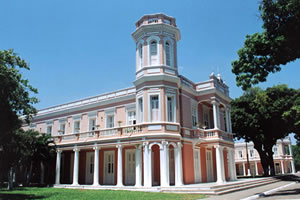
\includegraphics[width=16cm]{figuras/exemplo-1}
		}{
			\Fonte{\citeonline{UFC2012}.}
		}	
	\end{figure}
	
    Texto1 texto texto texto texto texto texto texto texto texto texto texto texto texto texto texto texto texto texto texto texto texto texto texto texto texto texto texto texto texto texto texto texto texto texto texto texto texto texto texto texto texto texto texto texto1.

    Texto2 texto texto texto texto texto texto texto texto texto texto texto texto texto texto texto texto texto texto. Texto texto texto texto texto texto texto texto texto texto texto texto texto texto texto texto texto texto texto2.

    Texto3 texto texto texto texto texto texto texto texto texto texto texto texto texto texto texto texto texto texto. Texto texto texto texto texto texto texto texto texto texto texto texto texto texto texto texto texto texto texto3.

    Texto4 texto texto texto texto texto texto texto texto texto texto texto texto texto texto texto texto texto texto. Texto texto texto texto texto texto texto texto texto texto texto texto texto texto texto texto texto texto texto4.

    A Figura \ref{fig:sondas} Texto texto texto texto texto texto texto texto texto texto texto texto texto texto texto texto texto texto texto. Texto texto texto texto texto texto texto texto texto texto texto texto texto texto texto texto texto texto texto3.

	\begin{figure}[h!]
		\centering
		\captionsetup{width=14cm}%Da mesma largura que a figura
		\Caption{\label{fig:sondas} Gráfico da Atmosfera Superior}	
		\UFCfig{}{
			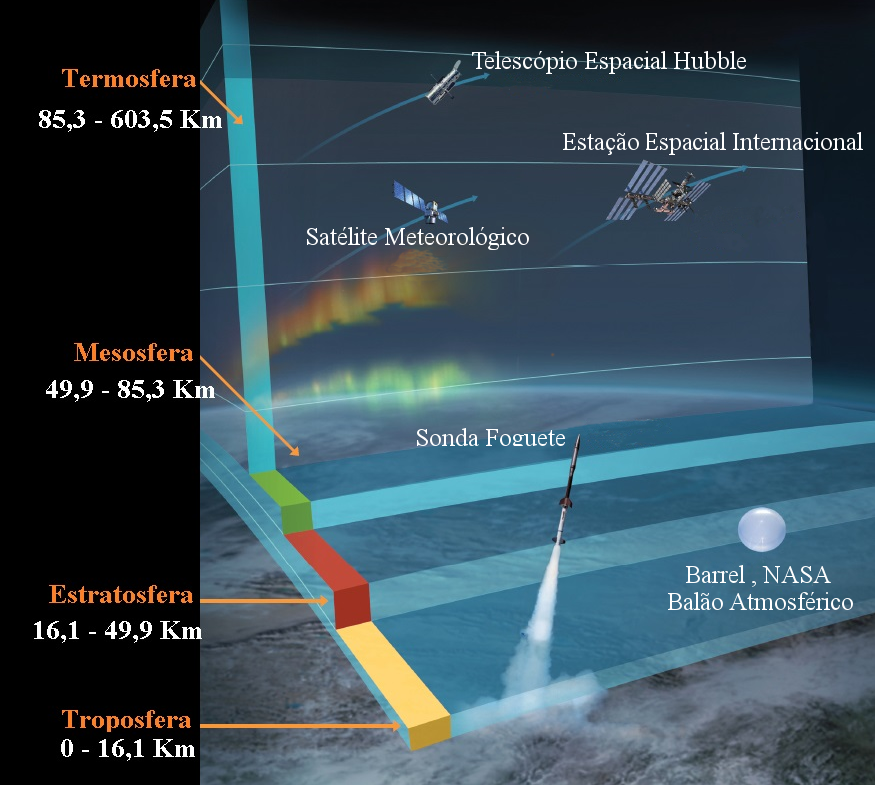
\includegraphics[width=14cm]{figuras/sondas}
		}{
			\Fonte{adaptado da \citeonline{NASA2016}.}}	
	\end{figure}

    Texto5 texto texto texto texto texto texto texto texto texto texto texto texto texto texto texto texto texto texto texto texto texto texto texto texto texto texto texto texto texto texto texto texto texto texto texto texto texto texto texto texto texto texto texto texto5.

    Texto6 texto texto texto texto texto texto texto texto texto texto texto texto texto texto texto texto texto texto texto texto texto texto texto texto texto texto texto texto texto texto texto texto texto texto texto texto texto texto texto texto texto texto texto texto5.

    Texto7 texto texto texto texto texto texto texto texto texto texto texto texto texto texto texto texto texto texto texto texto texto texto texto texto texto texto texto texto texto texto texto texto texto texto texto texto texto texto texto texto texto texto texto texto texto texto texto texto texto texto texto texto texto texto texto texto texto texto texto texto texto texto texto6.

    Evite terminar seções, capítulos e etc com figura. Procure escrever mais.

\section{Inserindo tabelas}\label{sec:tabelas}
    
    A Tabela \ref{tab:exemplo-1}... texto texto texto texto texto texto texto texto texto texto texto texto texto texto texto texto texto texto texto. Texto texto texto texto texto texto texto texto texto texto texto texto texto texto texto texto texto texto texto.
	
	\begin{table}[!h]
	\captionsetup{width=7cm}%Deixe da mesma largura que a tabela
	\Caption{\label{tab:exemplo-1} Um Exemplo de tabela alinhada que pode ser longa ou curta}%
	\IBGEtab{}{%
		\begin{tabular}{ccc}
			\toprule
			Nome & Nascimento & Documento \\
			\midrule \midrule
			Maria da Silva & 11/11/1111 & 111.111.111-11 \\
			Maria da Silva & 11/11/1111 & 111.111.111-11 \\
			Maria da Silva & 11/11/1111 & 111.111.111-11 \\
			\bottomrule
		\end{tabular}%
	}{%
	\Fonte{o autor.}%
	\Nota{esta é uma nota, que diz que os dados são baseados na
		regressão linear.}%
	\Nota[Anotações]{uma anotação adicional, seguida de várias outras.}%
    }
    \end{table}

	%\begin{table}[h!]	
	%	\centering
	%	\Caption{\label{tab:exemplo-1} Exemplo de tabela}	
	%	\UFCtab{}{
	%		\begin{tabular}{cll}
	%			\toprule
	%			Ranking & Exon Coverage & Splice Site Support \\
	%			\midrule \midrule
	%			E1 & Complete coverage by a single transcript & Both splice sites\\
	%			E2 & Complete coverage by more than a single transcript & Both splice sites\\
	%			E3 & Partial coverage & Both splice sites\\
	%			E4 & Partial coverage & One splice site\\
	%			E5 & Complete or partial coverage & No splice sites\\
	%			E6 & No coverage & No splice sites\\
	%			\bottomrule
	%		\end{tabular}
	%	}{
	%	\Fonte{elaborado pelo autor.}
	%}
	%\end{table}

\subsection{Exemplo de subseção} \label{sec:ex_sec}
	
    Texto texto texto texto texto texto texto texto texto texto texto texto texto texto texto texto texto texto texto texto texto texto texto texto texto texto texto texto texto texto texto texto texto texto texto texto texto texto texto texto texto texto texto texto texto.

    %acrlong{DATASUS},\acrlong{DNV},\acrlong{DO},\acrlong{ESF},\acrlong{IBGE},\acrlong{MFC},\acrlong{MI},\acrlong{MS},\acrlong{NV},\acrlong{ODM},\acrlong{OI},\acrlong{OMS},\acrlong{ONU},\acrlong{PNI},\acrlong{PSF},\acrlong{RIPSA},\acrlong{RN},\acrlong{SIM},\acrlong{SINASC},\acrlong{SUS},\acrlong{TMI},\acrlong{TMMFC}


    \begin{alineascomponto}
	    \item Integer non lacinia magna. Aenean tempor lorem tellus, non sodales nisl commodo ut
	    \item Proin mattis placerat risus sit amet laoreet. Praesent sapien arcu, maximus ac fringilla efficitur, vulputate faucibus sem. Donec aliquet velit eros, sit amet elementum dolor pharetra eget
	    \item Integer eget mattis libero. Praesent ex velit, pulvinar at massa vel, fermentum dictum mauris. Ut feugiat accumsan augue, et ultrices ipsum euismod vitae
	    \begin{subalineascomponto}
		    \item Integer non lacinia magna. Aenean tempor lorem tellus, non sodales nisl commodo ut
		    \item Proin mattis placerat risus sit amet laoreet.
	    \end{subalineascomponto}
    \end{alineascomponto}

\subsection{Uso de siglas} \label{sec:siglas}

    Para utilizar siglas, primeiro defina a sigla no arquivo "lista-de-abreviaturas-e-siglas"~ dentro da pasta "1-pre-textuais" com o comando 
    \begin{verbatim}
        \newacronym{ABNT}{ABNT}{Associação Brasileira de Normas Técnicas}
    \end{verbatim}
    Depois chame a sigla com o comando:
    \begin{verbatim}
        \gls{ABNT}
    \end{verbatim}
    Fica assim: \gls{ABNT}. A primeira vez que o comando é usado para uma determinada sigla, aparece o significado por extenso da sigla com a sua abreviação em seguida. A partir da segunda vez que o comando para uma determinada sigla é usado, aparace apenas a sigla. Por exemplo: \gls{ABNT}.  
    
    Veja o código fonte de outros exemplos: Teste de siglas \gls{TEST}, outros exemplos de siglas: \gls{DA}, \gls{MCEG}. 
    Repare que sempre as siglas estão sendo definidas primeiramente no arquivo ``lista-de-abreviaturas-e-siglas''.